\chapter{Analýza aplikace ve standardním podnikovém prostředí}
Aby aplikace byla v kontejnerovém prostředí škálovatelná, musí zároveň být distribuovatelná. Některé dnešní aplikace bohužel nelze převést do kontejnerů z důvodu špatné práce s pamětí. Tyto aplikace si uchovávají data v paměti a ukládají se na disk, až se aplikace zastaví. Migrovaná aplikace by měla být bezstavová.   

Aplikace je možné rozdělovat podle několika faktorů. Jedním z nich je stavovost, stavy definují jak služby a uživatelé komunikují se serverem. Z počátku většina webových aplikací byla bezstavová, jednalo se totiž o statické stránky, které měly velmi omezené možnosti interakce s koncovým uživatelem. S rozšířením webu se začal měnit přístup k webovým aplikacím na stavový model.

\section{Stavové aplikace (statefull)}
Stavová aplikace je taková aplikace, která udrží po dlouhou dobu otevřené spojení buď k uživateli, nebo k další službě. Pro tento typ aplikací musí být přizpůsobena řada komponent v infrastruktuře například databáze, webové servery, apod. Stavové aplikace jsou nejčastějším typem aplikací nacházejících se v podnikovém prostředí. Tyto aplikace musí mít striktně nastavené hostitelské prostředí, kde běží. Jejich největším problémem je špatná dynamika způsobená velkým množstvím závislostí na jednotlivých komponentách. Jeli aplikace vytížená, není ji možné škálovat a replikovat díky uchovávání stavů. Největší problém se škálováním je u databází .

\section{Bezstavové aplikace (stateless)}
Bezstavový přístup k aplikacím je vlastnost, která je v kontejnerovém světě zcela běžná. Díky této vlastnosti lze jednotlivé aplikace efektivně škálovat a šířit napříč vybranými platformami. Hlavní podstatou toho principu je přístupnost a komunikace mezi jednotlivými službami. Například: všechna data, se kterými aplikace pracují, by měla být ukládána v databázi, do které se aplikace bude připojovat. Databáze by neměla být závislá jen na jedné aplikaci, ale na celé řadě replik, které se vytvoří při škálování. 

Kontejnery jsou pouze jednotky, které vykonávají jednu činnost a neobsahují žádná data, proto bezstavový přístup povoluje kontejnerům nejen škálování, ale také rychlé vypínání a zapínání. Stavové aplikace jsou zejména doménou starého principu virtualizace, kdy se pro každou službu spouštěl jeden VM. Tyto aplikace bývají rovněž označovány jako legacy. Porovnání stavových a bezstavových architektur je na obrázku číslo \ref{fig:arch_app_statefull}.

\begin{figure}[H]
\begin{centering}
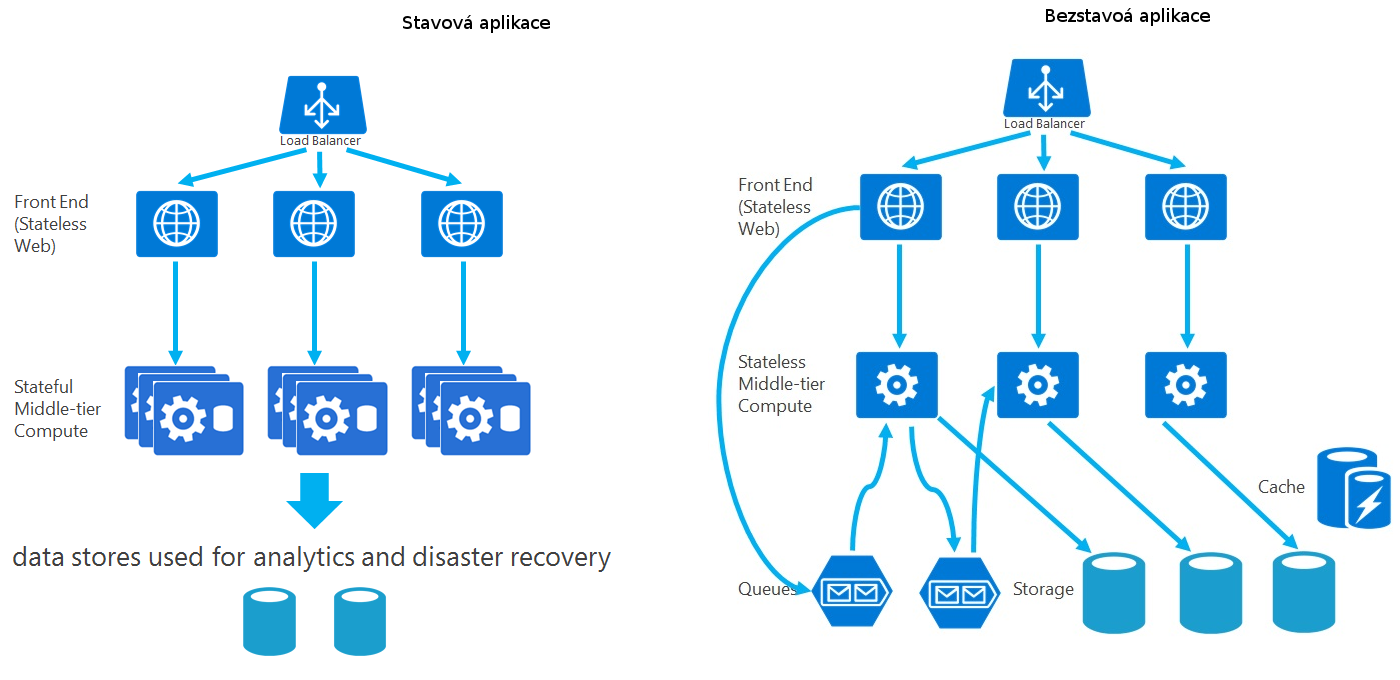
\includegraphics[width=1\textwidth]{img/micro_statefull}
\par\end{centering}
\caption{Rozdíl mezi stavovou a bezstavou aplikací z: \cite{ms_ms} \label{fig:arch_app_statefull}}
\end{figure}

\section{Architektura nekontejnerových aplikací}
Hlavní rozdíl mezi kontejnery a klasickým VM je v práci se zdroji. Tento problém byl již vysvětlen v kapitole číslo \ref{chp:kontejner}, nyní je třeba se zaměřit na architekturu aplikací běžících ve VM. Většina těchto nekontejnerových aplikací používá stavový přístup k datům. Služby tak nejsou specificky odděleny, například proxy server s sebou může nést více rolí z důvodu šetření zdrojů. Pro zachování principů vysoké dostupnosti musí být i VM přizpůsoben tak, aby při chybě na infrastruktuře aplikace fungovala i nadále. K tomu je nutné používat principy popsané v části \ref{par:ha} o vysoké dostupnosti. Problém se zdroji u VM je v jejich alokaci. Při spuštění VM se nastaví určité parametry, jako je počet jader, ram, hdd, a s těmito zdroji nelze dynamicky a efektivně pracovat. Většina virtualizačních technologií umí v reálném čase přidávat a snižovat tyto zdroje, ale samotné zvyšování znatelně ubírá výkon celému VM. Proto je vhodné alokovat pro dané VM dostatečné množství zdrojů a měnit je pouze v kritických situacích. Tím se běžně stává, že na serverech běží VM, které značně plýtvají se zdroji, protože je nedokáží plně využít.

\section{Popis aplikace}
Migrovaná aplikace v této práci je webová aplikace. V aplikaci byly použity komponenty Nginix, Memcached, MySql a OwnCloud. Celé schéma aplikace v kontejnerovém prostředí je zobrazeno na obrázku \ref{fig:arch_app_statefull}

Nginx je open source řešení pro webový server a reversní proxy. Koncept technologie Nginx je postaven na rychlé distribuci statického obsahu. Na rozdíl od Apache (webový server od Apache Foundation) vyřizuje všechny požadavky asynchronně. Mnohem častěji je však Nginx používán jako proxy server, který slouží například při přístupu z internetu do vnitřní sítě. Pomocí Nginxu lze nastavit řadu dalších nastavení, jako jsou limity připojených uživatelů na danou adresu, http/https redirecty, filtrace přístupů podle dané lokace atd. Nginx je jeden z nejrozšířenějších nástrojů pro web server/proxy na světě, využívají ho firmy jako Seznam.cz, Github či Dropbox\cite{ngnix}. 

Memcached je distribuovaný cache systém. Distribuovaná cache řeší problém při potřebě vyřídit požadavky při velkému přístupu uživatelů, díky tomuto řešení není potřeba upravovat část kódu aplikace či dokonce přidávat další hardware. Toto řešení je velmi podobné konkurenčnímu redisu, který je v praxi mnohem více rozšířen pro jeho jednoduchost. Hlavní důvod pro volbu memcached byla jeho multi-threadová podpora oproti redisu který dokáže pracovat pouze s jedním threadem. 

MySql je jedno z nejrozšířenějších open source řešení pro relační databáze. Velkou předností MySql je schopnost spouštění tohoto databázového řešení na všech dostupných platformách. Databáze se ovládá pomocí jazyka SQL. Mezi další výhody tohoto databázového řešení patří vysoká rychlost, jednoduché zálohovaní, apod. 

  %https://sysdig.com/blog/sysdig-docker-usage-report-2017/
Jako hlavní aplikace, která stojí mezi těmito open source projekty, byl zvolen OwnCloud. Owncloud je jednoduchá webová aplikace napsaná v programovacím jazyce PHP. Tato aplikace se zaměřuje na sdílení dat. OwnCloud je velmi podobný službám jako Google Drive, Dropbox. Hlavní výhodou je jeho otevřenost, díky otevřenému kódu řada vývojářů doimplementovala nové vlastnosti, jako jsou kalendáře, úprava tabulek a textových dokumentů, poznámky apod. Pro obsluhu OwnCloudu také lze používat mobilní aplikace, které byly oficiálně vydané firmou OwnCloud. 

Nevýhodou OwnCloudu je jeho oficiální podpora. Během minulého roku firmu opustila většina klíčových vývojářů, kteří si vytvořili nový projekt NextCloud (fork OwnCloudu). Podpora tohoto projektu tak zůstává převážně na komunitě uživatelů.


\begin{figure}[H]
\begin{centering}
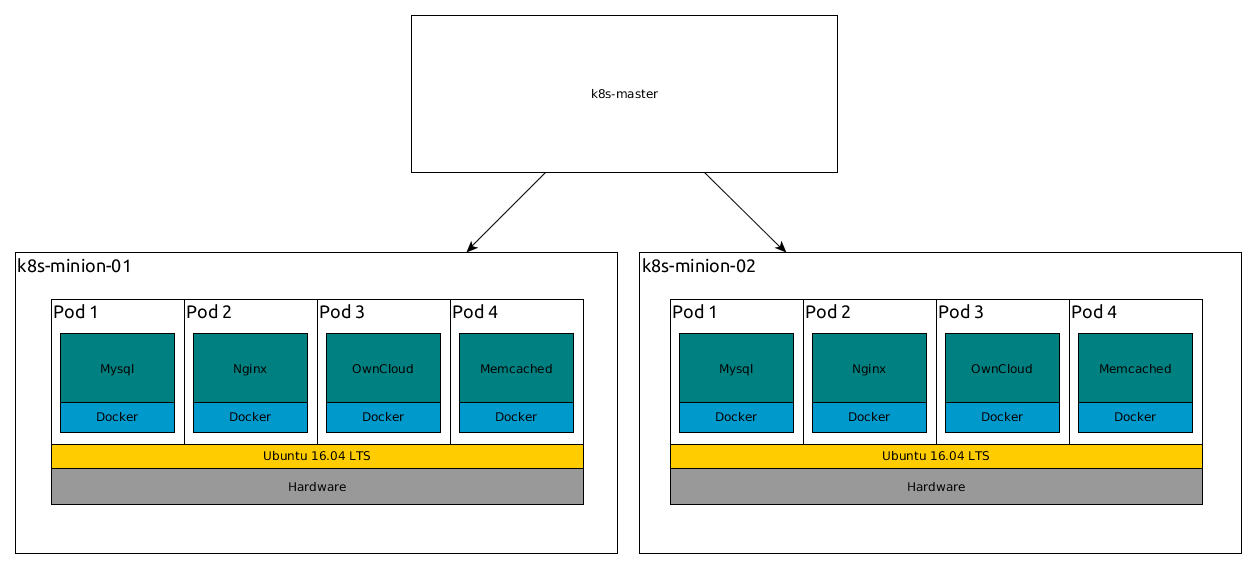
\includegraphics[width=1\textwidth]{img/k8schema}
\par\end{centering}
\caption{Architektura aplikace v kontejnerovém prostředí aplikací, zdroj: vlastní tvorba \label{fig:k8schema}}
\end{figure}


\section{Vybrané technologie}
V druhé a třetí kapitole byly představeny koncepty orchestrátorů a kontejnerů. Ve výběru je zohledněn faktor modularity a nahraditelnosti daného řešení. Každá infrastruktura měla být stavěna modulárně, aby bylo možno vyměnit jednotlivé komponenty bez větších změn.

\subsection{Kontejnerová technologie}
Pro kontejnerovou technologii je v práci použita technologie Docker, která je bezkonkurenčně nejrozšířenější. Byla zvolena převážně díky jednoduché tvorbě nových kontejnerů a díky snadnější práci s vrstvícím systémem. Další výhodou je vestavěný systém na práci s images, který Docker implementuje. Zároveň lze velmi jednoduše propojit s repositářem po ukládání těchto images.
Výhodou Docker images je jejich znovupoužitelnost. Jakmile je image sestavený, lze ho volně převést na rkt kontejner. Pro kompatibilitu lze také využít rkt runtime, který dokáže rovněž spouštět a provozovat Docker kontejnery. 

\subsection{Orchestátor}
Pro praktickou část je zvolen orchestártor Kubernetes. Splňuje všechny požadavky, jako jsou vysoká dostupnost, škálovatelnost a life-cycle-management. Jelikož praktická část je zaměřena především na modularitu, výběr byl omezen pouze na orchestrátory Mesos a Kubernetes. 

Mesos nebyl zvolen, protože se jedná o nástroj, který není zaměřen pouze na kontejnery a pro jeho instalaci je důležité vyřešit spoustu dalších otázek (například nastavení zookeeperu). Tento nástroj je vhodné řešení zejména pro celá datová centra, kde dokáže efektivně řídit zdroje. Pro potřeby menších clusterů je příliš těžkopádný a složitý.

Kubernetes ve své architektuře implementuje postupy, které by se mohly nazývat automatické léčení (self-healing). Orchestrátor dokáže ve stanoveném čase reagovat na podněty, jako jsou pády kontejnerů a služeb. V případě poruchy je schopen obnovit chybějící části aplikace na jiné části infrastruktury. Všechny tyto operace se mohou provádět především díky  distribuované architektuře Kubernetes. 

Rozšiřitelnost stávajícího clusteru je také důležitý prvek, ve velkých systémech je nežádoucí, aby přidávání nového hardwareru bylo složité a zdlouhavé. V Kubernetes rozšiřování funguje velmi jednoduše, stačí na daném zařízení nastavit roli, kterou má vykonávat, a předat informaci o novém serveru Kubernetes masteru. Všechny dodatečné procesy jako adresování a spouštění nových kontejnerů si Kubernetes určí sám. 
